\documentclass[reqno]{amsart}
\usepackage{amscd, amssymb, amsmath, amsthm}
\usepackage{graphicx}
\usepackage[colorlinks=true,linkcolor=blue]{hyperref}
\usepackage[utf8]{inputenc}
\usepackage[T1]{fontenc}
\usepackage{textcomp}
\usepackage{babel}
%% for identity function 1:
\usepackage{bbm}
%%For category theory diagrams:
\usepackage{tikz-cd}


\setlength\parindent{0pt}

\pdfsuppresswarningpagegroup=1

\newtheorem{theorem}{Theorem}[section]
\newtheorem{lemma}[theorem]{Lemma}
\newtheorem{proposition}[theorem]{Proposition}
\newtheorem{corollary}[theorem]{Corollary}
\newtheorem{conjecture}[theorem]{Conjecture}

\theoremstyle{definition}
\newtheorem{definition}[theorem]{Definition}
\newtheorem{example}[theorem]{Example}
\newtheorem{exercise}[theorem]{Exercise}
\newtheorem{problem}[theorem]{Problem}
\newtheorem{question}[theorem]{Question}

\theoremstyle{remark}
\newtheorem*{remark}{Remark}
\newtheorem*{note}{Note}
\newtheorem*{solution}{Solution}



%Inequalities
\newcommand{\cycsum}{\sum_{\mathrm{cyc}}}
\newcommand{\symsum}{\sum_{\mathrm{sym}}}
\newcommand{\cycprod}{\prod_{\mathrm{cyc}}}
\newcommand{\symprod}{\prod_{\mathrm{sym}}}

%Linear Algebra

\DeclareMathOperator{\Span}{span}
\DeclareMathOperator{\Ima}{Im}
\DeclareMathOperator{\diag}{diag}
\DeclareMathOperator{\Ker}{Ker}
\DeclareMathOperator{\ob}{ob}
\DeclareMathOperator{\Hom}{Hom}
\DeclareMathOperator{\Mor}{Mor}
\DeclareMathOperator{\sk}{sk}
\DeclareMathOperator{\Vect}{Vect}
\DeclareMathOperator{\Set}{Set}
\DeclareMathOperator{\Group}{Group}
\DeclareMathOperator{\Ring}{Ring}
\DeclareMathOperator{\Ab}{Ab}
\DeclareMathOperator{\Top}{Top}
\DeclareMathOperator{\hTop}{hTop}
\DeclareMathOperator{\Htpy}{Htpy}
\DeclareMathOperator{\Cat}{Cat}
\DeclareMathOperator{\CAT}{CAT}
\DeclareMathOperator{\Cone}{Cone}
\DeclareMathOperator{\dom}{dom}
\DeclareMathOperator{\cod}{cod}
\DeclareMathOperator{\Aut}{Aut}
\DeclareMathOperator{\Mat}{Mat}
\DeclareMathOperator{\Fin}{Fin}
\DeclareMathOperator{\rel}{rel}
\DeclareMathOperator{\Int}{Int}
\DeclareMathOperator{\sgn}{sgn}
\DeclareMathOperator{\Homeo}{Homeo}
\DeclareMathOperator{\SHomeo}{SHomeo}
\DeclareMathOperator{\PSL}{PSL}
\DeclareMathOperator{\Bil}{Bil}
\DeclareMathOperator{\Sym}{Sym}
\DeclareMathOperator{\Skew}{Skew}
\DeclareMathOperator{\Alt}{Alt}
\DeclareMathOperator{\Quad}{Quad}
\DeclareMathOperator{\Sin}{Sin}
\DeclareMathOperator{\Supp}{Supp}
\DeclareMathOperator{\Char}{char}
\DeclareMathOperator{\GL}{GL}
\DeclareMathOperator{\codim}{codim}


%Row operations
\newcommand{\elem}[1]{% elementary operations
\xrightarrow{\substack{#1}}%
}

\newcommand{\lelem}[1]{% elementary operations (left alignment)
\xrightarrow{\begin{subarray}{l}#1\end{subarray}}%
}

%SS
\DeclareMathOperator{\supp}{supp}
\DeclareMathOperator{\Var}{Var}

%NT
\DeclareMathOperator{\ord}{ord}

%Alg
\DeclareMathOperator{\Rad}{Rad}
\DeclareMathOperator{\Jac}{Jac}

%Misc
\newcommand{\SL}{{\mathrm{SL}}}
\newcommand{\mobgp}{{\mathrm{PSL}_2(\mathbb{C})}}
\newcommand{\id}{{\mathrm{id}}}
\newcommand{\Mod}{{\mathrm{Mod}}}
\newcommand{\PMod}{{\mathrm{PMod}}}
\newcommand{\SMod}{{\mathrm{SMod}}}
\newcommand{\ud}{{\mathrm{d}}}
\newcommand{\Vol}{{\mathrm{Vol}}}
\newcommand{\Area}{{\mathrm{Area}}}
\newcommand{\diam}{{\mathrm{diam}}}
\newcommand{\End}{{\mathrm{End}}}


\newcommand{\reg}{{\mathtt{reg}}}
\newcommand{\geo}{{\mathtt{geo}}}

\newcommand{\tori}{{\mathcal{T}}}
\newcommand{\cpn}{{\mathtt{c}}}
\newcommand{\pat}{{\mathtt{p}}}

\let\Cap\undefined
\newcommand{\Cap}{{\mathcal{C}}ap}
\newcommand{\Push}{{\mathcal{P}}ush}
\newcommand{\Forget}{{\mathcal{F}}orget}





\begin{document}

\section{Glossary for exam}

\begin{itemize}
    \item All subspaces have a complement (thm 2.14)
    \item $A,\tilde{A}\in \Hom (U,V)$ are equivalent if there
        exist $S \in \GL (U)$ and $T \in \GL (V)$ such that
         \begin{equation*}
        \begin{tikzcd}
            U  \ar[r, "A"] \ar[d, "S"] & V \ar[d, "T"] \\
            U \ar[r, "\tilde{A}"] & V
        \end{tikzcd}
        \end{equation*}
    \item $A,\tilde{A} \in \End(V)$ are called similar if
        there exists $T \in \GL (V)$ such that
        $TA = \tilde{A}T$.
    \item \textbf{Theorem 2.22:} Assume $U,V$ fin.dim., then
        $A, \tilde{A}$ are equivalent iff they have the same rank.
    \item For $y \in V'$, the null-space of $y$ has codimension
        one in $V$ and only the non-zero scalar multiples
        of $y$ have the same null-space as $y$. (lemma 3.15 + see 
        thm 3.14)
    \item The dual map is the pullback: if $A \in \Hom (U,V)$, then
        $A' \in \Hom(V',U')$ is defined by
        $A'(y) = y \circ A$.
       \begin{equation*}
        \begin{tikzcd}
            U \ar[r, "A"] \ar[dr, "A'(y)"']& V \ar[d, "y"] \\
              & k
        \end{tikzcd}
        \end{equation*}
    \item $\Bil (V) \cong M_{n,n}(F)$ when $\dim V = n$ through
        the isomorphism
        $B \stackrel{\cong}{\mapsto} \left( B(x_i,x_j) \right) $.
        $\Bil (V)$ has basis $w_{i,j} = y_i y_j$ where
        $\left( y_i \right) $ is a dual basis to a basis
        $\left( x_i \right) $ for $V$ and
        $\left( y_iy_j \right) (x,z) = y_i(x) y_j(z)$.
    \item $L^{k}(V) :=
        \left\{ \text{multilinear forms }
        V^{\times k} \to  F \right\} $.
    \item Review chapter 4 again - bilinear, symmetric,
    skew-symmetric, alternating, quadratic forms.
\item Polynomials $p(x) \in F[x]$ are uniquely determined
    by their associated functions
    $\lambda \mapsto p(\lambda)$ if and only if
    $F$ is infinite.
\item When $A$ is diagonable, the projections
    $E_{\lambda} \colon V \to V_{\lambda}$ are called
    the spectral projections of $A$ and the
    expansion of $A$ as
    $A = \sum_{\lambda \in \sigma(A)}
    \lambda E_{\lambda}$ is called the spectral resolution of
    $A$.
\item Using Gram-Schmidt, we find that every finite-dimensional
    inner product space has an orthonormal basis.
\item Fitting's decomposition shows that
    all endomorphisms act on $V$ by a nilpotent map on
    one subspace $N$ and an invertible map on another subspace $R$,
    and
    these subspaces form a unique direct sum reduction
    $V = N \oplus R$.
\item All transpositions are conjugate in $S_n$ and every
    permutation is a product of transpositions. 
\item Bruhat decomposition shows that
    every isomorphism is the product
    $S T U$ of invertible upper triangular matrices
    $S$ and $U$ and a permutation matrix $T$.
\item $LU$-decomposition is just a different form of Bruhat
    decomposition: for $A \in \GL(n,F)$, there
    exist matrices $L,P,U$ such that
    $A = LPU$ with $L$ lower triangular, $U$ upper triangular,
    and $P$ a permutation matrix.
\item By the Jordan additive decomposition, for
    $A \in \End(V)$, it splits uniquely as
    $A = A_d + A_n$ where $A_d$ is diagonable and
    $A_n$ is nilpotent. 
    Moreover, $\sigma(A_d) = \sigma(A)$ and there
    exist $p_d,p_n \in F[x]$ such that
    $p_d(A) = A_d$ and $p_n (A) = A_n$.
\item Lemma 13.11: Assume $A \ge 0$ and
    $A^{m} > 0$ for some $m \in \mathbb{N} $. If a vector
    $x \ge 0$ satisfies $Ax \ge \rho x$ then
    $Ax = \rho x$.
\end{itemize}


\section*{Chapter 1}

\section*{Chapter 4}
    
\begin{exercise}[1]
    How does the matrix $\left[ B \right] $ representing a bilinear
    form transform if the basis is changed by a 
    transition matrix $\left[ P \right] $?
\end{exercise}

\begin{solution}
    Suppose $\mathcal{B}=
    \left\{ x_1, \ldots, x_n \right\} $ is the
    basis for $V$ giving $\left[ B \right] $ the representation.
    Write $\left[ B \right]_{\mathcal{B}}
    = \left( B(x_i, x_j) \right) $ for this representation.
    We can write
    \[
    B = \sum B(x_i,x_j) w_{ij}.
    \] 
    Let $P$ be a change of basis sending 
     $x_j \mapsto \sum_{i} P_{ij} v_i$ and
     let $\mathcal{B}' = \left\{ v_1, \ldots, v_n \right\} $.
     Suppose $\left( z_i \right) $ is the dual
     basis to $\mathcal{B}'$ and
     $\tilde{w}_{ij}= z_i z_j$.
     Then
     \[
     B = \sum B \left( v_i, v_j \right) \tilde{w}_{ij}.
     \] 
     So $\left[ B \right]_{\mathcal{B}'}=
     \left( B\left( v_i,v_j \right)  \right) $.
     Now
     \begin{align*}
     B\left( x_i , x_j \right) = 
     \sum B \left( v_s, v_t \right) \tilde{w}_{s,t}
     \left( P(x_i), P(x_j) \right) 
     &= \sum B\left( v_s, v_t \right) \tilde{w}_{s,t}
     \left( \sum P_{ki}v_k, \sum P_{rj} v_r \right)\\
     \sum_{s,t} B (v_i, v_j) P_{si } P_{tj}
     \end{align*}
\end{solution}

\begin{exercise}[4.7]
    Determine the symmetric bilinear form on
    $\mathbb{R}^2$ corresponding
    to the quadratic form
    $q(x) = 2x_1^2 + 6x_1x_2 - 3x_2^2$. Find a basis for
    which $q$ has the form
    \[
    ax_1^2 + bx_2^2.
    \] 
\end{exercise}

\begin{solution}
    The symmetric bilinear form
    $B(\left( x_1,x_2 \right), \left( y_1,y_2 \right) )
    = 2x_1 y_1 + 3x_1 y_2 + 3 x_2 y_1 - 3 x_2 y_2$ works.
    The bilinear form is given the matrix
    $\left[ B \right] =
    \begin{pmatrix} 2 & 3 \\ 3 & -3 \end{pmatrix} $ where
    $B(x,y) = x^{t} \left[ B \right] y$.

    Now setting up
    \[
        \begin{pmatrix} 2 & 3 & x_1\\
        3 & -3 & x_2 \end{pmatrix} 
    \] 
    this is equivalent to the matrix
    \[
        \begin{pmatrix}    1 & 0 & \frac{x_2}{5}+x_1\\
        0 & 1 & \frac{3x_1 - 2x_2}{15}
\end{pmatrix}
    \] 
    So choosing a basis as
    $\mathcal{B}' = \left\{ y_1,y_2 \right\} $ with
    $y_1 = \frac{x_2}{5}+x_1$ and
    $y_2 = \frac{3x_1-2x_2}{15}$, we get
    \[
    q(y) = y^{t} \left[ B \right]_{\mathcal{B}'}
    y = y_1^2 + y_2^2.
    \] 
\end{solution}


\section*{Chapter 5}

\begin{exercise}[5.4]
    $X,Y \subset V$ subspaces,
    $A \colon V \to V /X \oplus V / Y$ by
    $v \mapsto \left( v+X,v+Y \right) $ and
    $B \colon V / X \oplus V /Y \to 
    V / X+Y$ given by
    $\left( v_1+X,v_2+Y \right) \mapsto 
    v_1-v_2 + \left( X+Y \right) $.
    Give a codimension version of the Grassmann formula.
\end{exercise}

\begin{solution}
    Firstly, $N(A) = X \cap Y$, and
    $R(B) = V / \left( X+Y \right) $ since
    for $v + \left( X+Y \right)$, we have
    $B \left( v+X, 0+Y \right) =
    v+\left( X+Y \right) $. Now
    if $B\left( v_1+X,v_2+Y \right) =
    v_1-v_2 + \left( X+Y \right) = 0 + \left( X+Y \right) $ then
    $v_1- v_2 \in X+Y$ so
    $v_1-v_2 = x+y$ and hence
    $v := v_1-x = y+v_2$, so
    $A(v) = \left( v+X, v+Y \right) 
    = \left( v_1+ X, v_2 + Y \right) $, hence
    $N(B) \subset R(A)$, but also,
    $R(A) \subset N(B)$ clearly. Hence
    $N(B) = R(A)$. Now by rank-nullity, we get
    \begin{align*}
    \codim X + \codim Y 
    &=
    \codim \left( X+Y \right) + N(B)\\
    &= \codim (X+Y) + \dim V - \dim \left( X \cap Y \right)\\
    &= \codim (X+Y) + \codim \left( X \cap Y \right) 
    \end{align*}
    \qed
\end{solution}

\section*{Chapter 6}

\begin{figure}[htpb]
    \centering
    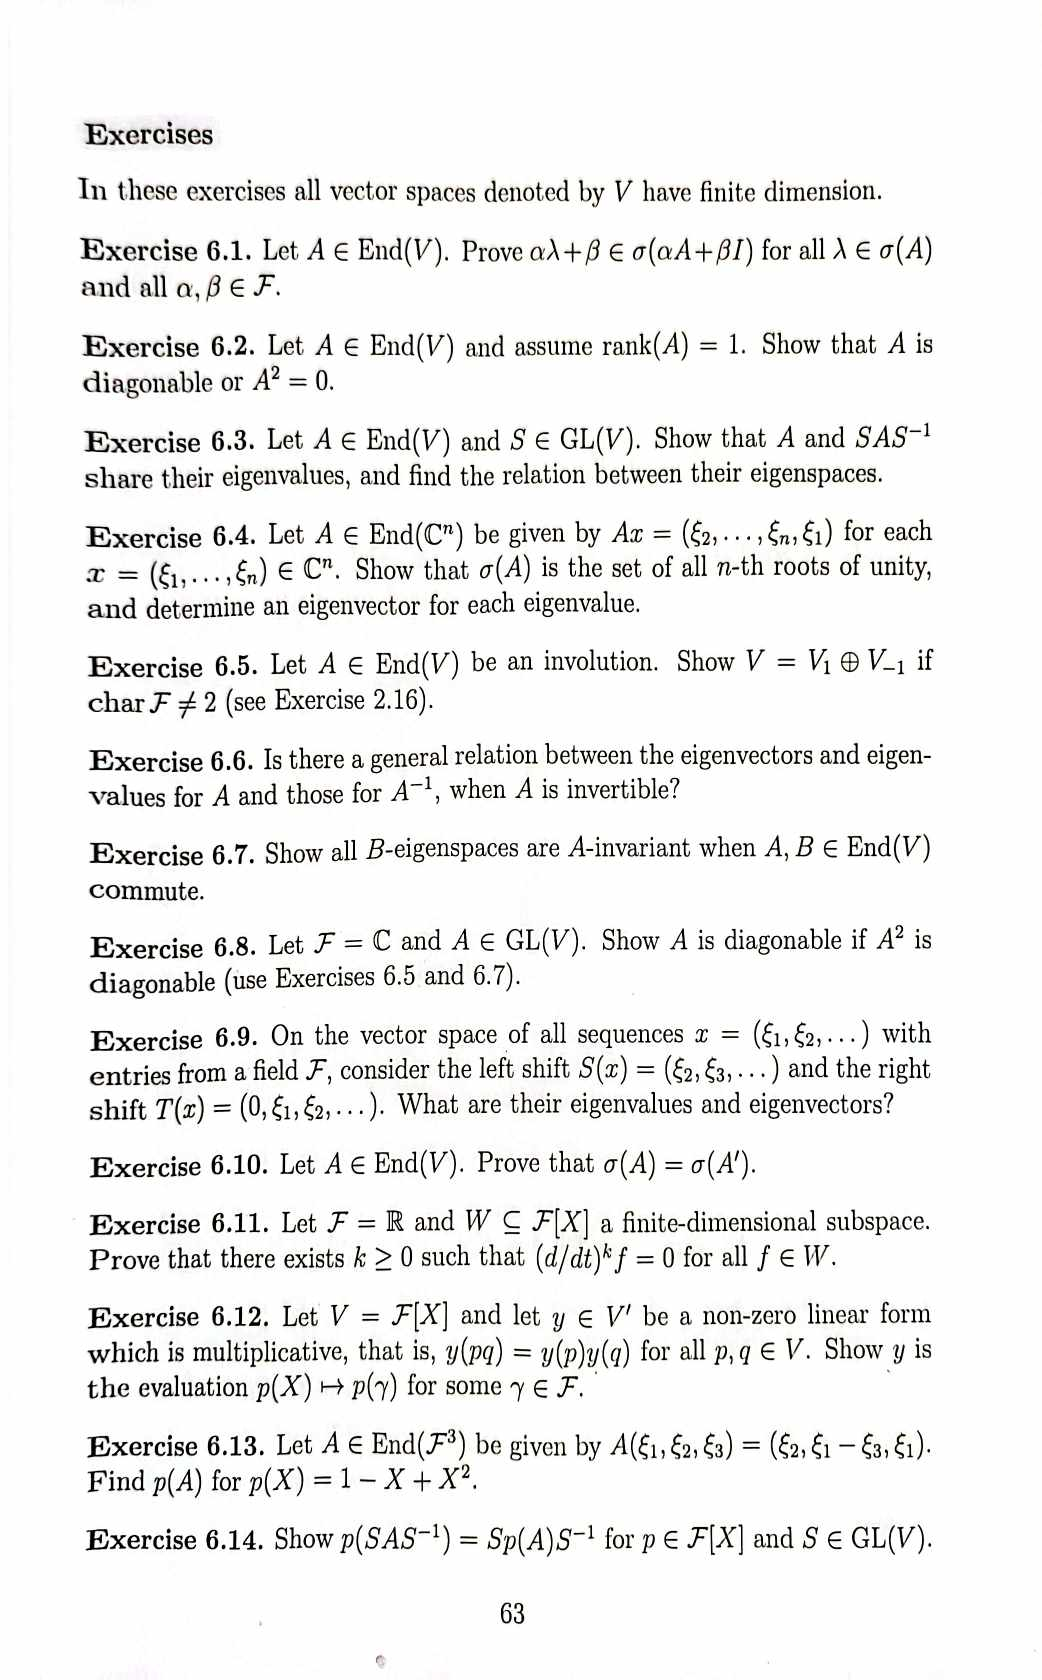
\includegraphics[width=0.8\textwidth]{chapter-6-exercises.jpg}
\end{figure}

\section*{Chapter 7}



\section*{Chapter 12}

\begin{exercise}[12.2]
    Let $U$ and $V$ be normed spaces, and assume that $V$ is complete.
    Show that then $B(U,V)$ is also complete with the operator
    norm.
\end{exercise}

\begin{solution}
    Suppose $B_n$ is a Cauchy sequence
    in $B \left( U,V \right) $, so
    \[
    \forall \varepsilon > 0 \exists N \in \mathbb{N}  \mid 
    \|B_n - B_m\|< \varepsilon, \quad \forall m,n \ge N.
    \] 

    That is, for all $m, n \ge N$,
    \[
    \sup_{\|x\|= 1} \|B_n x - B_m x \| < \varepsilon
    \] 
    For a fixed $n$, this becomes a Cauchy sequence
    in $V$ which thus converges, so we can define
    $Bx = \lim_{n \to \infty} B_n x$.
    We claim that $B$ is a bounded operator too.
    It is clear that it is linear since each $B_n$ is a 
    continuous map. What remains is to show that
    $B$ is bounded. It suffices to show that
    it is bounded on $ S = \left\{ x  \mid \|x \|= 1 \right\} $.
    Suppose it were not bounded and choose
    a sequence $\left( x_n \right) \subset S$ such that
    $\|Bx_n\|> n$.
    Choose $\varepsilon = \frac{1}{2}$ and let
    $N$ be such that for $n, m \ge N$, we have
    \[
    \|B_n - B_m\|< \varepsilon
    \] 
    Then for all $k$
    \[
    \|B_n x_k -  B_m x_k \|< \varepsilon
    \] 
    for all $n \ge N$, so in particular
    \[
    \|Bx_k - B_m x_k\|
    = \lim_{n \to \infty} \|B_n x_k -  B_m x_k \|< \varepsilon
    \] 
    But $B_m$ is bounded, so let $\|B_m\| = R$.
    Choose $M$ such that that for all $k \ge M$, we have
    $\|Bx_k \| \ge \|B_m x_k\|$, then
    \[
    \|B x_k\| - \|B_m x_k\| < \varepsilon
    \] 
    giving
    \[
    \|B x_k\| < \varepsilon + R
    \] 
    contradicting $\|Bx_k\| \to \infty$.

\end{solution}

    \begin{exercise}[12.3]
        Let $A \in B(V)$ for a complete normed space
        $V$. Prove
        \begin{enumerate}
            \item If $\|A\| < 1$ then
                $\sum_{k=0}^{\infty} A^{k}$ converges
                in $B(V)$ to an inverse of $I - A$.
            \item If $B \in B(V)$ is invertible and
                $\|A\| < \frac{1}{\|B^{-1}\|}$ then
                $B - A$ is invertible.
            \item The set of invertible bounded operators is an
                open subset of $B(V)$.
        \end{enumerate}
        (Here invertible means there is a bounded inverse)
    \end{exercise}

    \begin{solution}
        (1) geometric series.

        (2) $B - A = B \left( 1 - \frac{A}{B} \right) $.
        Now $\|\frac{A}{B}\| \le 
        \|A\| \|B^{-1}\| < 1$, so
        by (1),  $1 - \frac{A}{B}$ has inverse
        $\sum_{k=0}^{\infty} \left( \frac{A}{B} \right)^{k}$.
        But then $B - A$ is a composition of invertible
        maps hence invertible since $\text{GL} (V)$ is a group.

        (3) Suppose 
        $A \in B\left( B, \frac{1}{\|B^{-1}\|} \right) $, so
        $\| B - A\| < \frac{1}{\|B^{-1}\|}$. By (2), 
        $B - (B-A) = A$ is then invertible. Hence
        $B \left( B, \frac{1}{\|B^{-1}\|} \right) $ is an
        open neighborhood of $B$ in $B(V)$ consisting
        of invertible maps. Thus the
        set of invertible maps is open in $B(V)$.
    \end{solution}

    \begin{exercise}[12.6]
        Let $S \in \End \left( \ell^2 \right) $ denote the
        right shift taking the sequence
        $\left( x_1, x_2, \ldots \right) $  to
        $\left( 0, x_1, x_2, \ldots \right) $. Show it
        is bounded and determine the operator
        norm $\|S\|$. Find also the adjoint $S^{*}$, and
        verify that $S^{*}S = I$ but
        $S S^{*} \neq I$.
    \end{exercise}

    \begin{solution}
        Recall that we are dealing with the norm
        $\| \left( x_1, x_2, \ldots \right) \|^2
        = \sum_{k=1}^{\infty} \left| x_k \right|^2 $.
        But indeed then if
        $\|\left( x_1, \ldots \right) \| = 1$, then
        \[
        \|S \left( x_1, \ldots \right) 
        \|^2 = 
        \| \left( 0, x_1, x_2, \ldots \right) \|^2
        = \sum_{k=1}^{\infty} \left| x_k \right|^2
        = 1
        \] 
        so, in fact, $S$ preserves the norm.
        But then
        since $\|S x\| = \|x\|$ for all $x$ by linearity, we have
        $\|S\| = 1$.
        Now, the inner product is
        $\left<x,y \right> = 
        \sum_k x_k \overline{y_k}$. Then
        \[
        \left< Sx,y \right>
        = \sum_{k=2}^{\infty} x_{k} y_{k-1} =
        \left< x, S^{*}y \right>
        \] 
        if we define $S^{*}\left( y_1, y_2, \ldots \right) 
        = \left( y_2, y_3 , \ldots \right) $.
        We then indeed get
        $S^{*}S = I$ clearly, but
        $S S^{*} \left( x_1,x_2,  \ldots \right) 
        = \left( 0, x_2, x_3, \ldots \right) $.
    \end{solution}

    \begin{exercise}[12.8]
        Show $\|Ax \pm ix\|^2 = 
        \|Ax\|^2 + \|x\|^2 $ for $A$ Hermitian
        and $\dim V < \infty$. Then show
        $A \pm i I$ is invertible and
        $\left( A - i I \right) \left( A+iI \right)^{-1}$ 
        unitary.
    \end{exercise}

    \begin{solution}

        \begin{align*}
        \left<Ax \pm ix, Ax \pm ix \right> 
        &=
        \|Ax\|^2 + \left< Ax , \pm ix \right>
        + \left< \pm ix, Ax \right>
        + \left<\pm ix, \pm ix \right>
        \\
        &= \|Ax\|^2 + \|x\|^2
        \mp i \left<Ax , x \right>
        \pm i \left< x, Ax \right>\\
        &= \|Ax\|^2 + \|x\|^2
        \mp i \left<Ax,x \right>
        \pm i \left<Ax,x \right>\\
        &= \|Ax\|^2 + \|x\|^2.
        \end{align*}

        Now, if $A \pm i I$ were not invertible, it
        would not be injective, so for 
        $x \neq 0$, we would get
        \[
        0 = \|Ax \pm i x\|^2
        = \|Ax\|^2 + \|x\|^2
        \] 
        but $\|x\|^2 > 0$ and
        $\|Ax\|^2 \ge 0$, so this gives a contradiction.

        Lastly, what is the adjoint of
        $\left( A-iI \right) \left( A+iI \right)^{-1}$?
        Well, $\left( A-iI \right)^{*}
        = A + iI$ by the rules on page 70. Hence
        the expression is of the form
        $X^{*} X^{-1}$ which has adjoint
        $\left( X^{-1} \right)^{*} X$. Then
        $\left( X^{-1} \right)^{*} X X^{*} X^{-1}$.


        Now, since $A$ is self-adjoint, it is in particular
        normal, so $A + iI$ is normal and
        hence orthogonally diagonable. Writing
        $A+ iI = \sum \lambda E_{\lambda}$, we get
        $(A+iI)^{*} = \sum \overline{\lambda} E_{\lambda}$, so
        $A+iI$ and $A-iI$ commute. Hence we get
         $X X^{*} = X^{*} X$, and the expression above becomes
         the identity.
    \end{solution}



    \begin{exercise}[12.4]
        Give a simple proof of the Hahn-Banach theorem for
        a continuous linear form on a closed subspace of
        a Hilbert space.
    \end{exercise}

    \begin{solution}
        Let $V$ be a Hilbert space and let
        $U \subset V$ be a closed subspace. Then
        $V = U \oplus U^{\perp}$. Let
        $\mathcal{B}$ be a basis for
        $U$ and extend it to a basis 
        $\mathcal{A}$ for $V$. Take the duals
        $\mathcal{B}^{'}$ and $\mathcal{A}^{'}$.
        For $z \in U^{*}$ we can write
        $z = \sum_{y_i' \in \mathcal{B}'}
        a_i y_i$. Then $z$ can also be considered a linear
        form on $V$ by letting the coefficient for
        $y_i \in \mathcal{A}'$ be $0$ if
        $y_i \not\in \mathcal{B}'$ and
        $a_i$ otherwise. The restrictions are clearly
        the same. 
        By the Riesz-Fréchet representation theorem,
        since $U$ is a closed subspace of a Hilbert space, it
        is also a Hilbert space, so by continuity of $z$, there
        exists $u \in U$ such that
        $z(x) = \left< x,u \right>$ for all $x \in U$ and
        such that $\|z\| = \|u\|$.
        But since  $z|_{U^{\perp}} = 0$, we also
        have $z(x) = \left< x,u \right>$ for all $x \in V$, so
        by the Riesz-Fréchet theorem, $\|z\| = \|u\|$ over $V$ as well.


    \end{solution}


    \begin{exercise}[13.1]
        Prove $\rho (A+B) \le \rho (A) + \rho(B)$ if
        $A$ and $B$ are normal. Prove it for general
        $A,B \in \End (V)$, now assuming they commute.
        Show the inequality can fail in general.
    \end{exercise}

    \begin{solution}
        
        If $A$ and $B$ are normal, then
        they are orthogonally diagonable with respect
        to the associated inner product, hence
        $\rho (A) = \|A\|$ and
        $\rho(B) = \|B\|$.
        Now, in general, we have
        $\rho(X) \le \|X\|$, we we get
        \[
        \rho(A+B) \le \|A+B\|
        \le \|A\| + \|B\|
        = \rho(A) + \rho(B).
        \] 


        If $A$ and $B$ commute, then
        \begin{align*}
        \rho(A+B) = 
        \lim_{k\to \infty}
        \|\left( A+B \right)^{k}\|^{\frac{1}{k}}
        &=
        \lim_{k\to \infty}
        \| \sum_{i=0}^{k} \begin{pmatrix} k\\i \end{pmatrix} 
        A^{i} B^{k-i} \|^{\frac{1}{k}}\\
        &\le \lim_{k\to \infty}
        \left| \sum_{i=0}^{k} 
        \begin{pmatrix} k\\i \end{pmatrix} 
        \|A\|^{i} \|B\|^{k-i} \right|^{\frac{1}{k}}\\
        &= \lim_{k\to \infty} 
         \|A\|+\|B\|\\
        &= \|A\| + \|B\|\\
        &= \lim_{k\to \infty} \|A^{k}\|^{\frac{1}{k}} +
        \lim_{k\to \infty} \|B^{k}\|^{\frac{1}{k}}
        \end{align*}
        where the last equality follows from
        $\|X^{k}\| = \|X\|^{k}$ when $X$ is diagonable (by
        the proof of lemma 13.4).




        To show that it can fail in general, note that
        for $\left[ A \right] =
        \begin{pmatrix} 1 & 0 \\ 1 & 1\end{pmatrix} $ and
        $\left[ B \right] =
        \begin{pmatrix} 1 & 1\\
        0 & 1\end{pmatrix} $, we have
        that the eigenvalues of both are precisely
        $1$, hence $\rho(A) + \rho(B) = 2$, while
            $A+B = \begin{pmatrix} 2 & 1\\
            1 & 2\end{pmatrix} $ which has characteristic
            polynomial
            $(x-3)(x-1)$ and thus
             $3$ as an eigenvalue.
    \end{solution}





    \begin{exercise}[13.2]
        Let $F = \mathbb{C}$. Find a counterexample to the
        statement:
        $\rho \left( p \left( A \right)  \right) 
        = p \left( \rho(A) \right) $ for all polynomials
        $p$, where $\rho$ is the spectral radius. 
    \end{exercise}

    \begin{solution}

        Consider $p(x) = ix - i$ and
        $A = -I$. So
        $p(A) = \begin{pmatrix} -2i &0 \\0 & -2i \end{pmatrix} $ 
        which has spectral radius
        $2$. However,
        $-I$ has spectral radius $1$ and
        $p(1) = 0$.
    \end{solution}

    \begin{exercise}[13.3]
        Show $\rho \left( A^{*}A \right) 
        = \|A^{*}A\| = \|A\|^2$ for the
        operator
        norm of an inner product.
    \end{exercise}


    \begin{solution}
        The first equality holds when
        the matrix is orthogonally diagonable.
        But  $A^{*}A$ is self-adjoint, hence
        normal hence orthogonally diagonable.

        The latter equality holds since
        \[
        \|A^{*}A\| =
        \sup_{\|x\|=1} \left<A^{*}Ax, x \right>
        = \sup_{\|x\|=1} \|Ax\|^2
        = \|A\|^2
        \] 
    \end{solution}



























    %\bibliography{../refs.bib}
\end{document}
